\documentclass[11pt,a4paper]{article}
% Generated with LaTeXDraw 2.0.8
% Sat Nov 05 14:57:05 EDT 2011
\usepackage[usenames,dvipsnames]{color}
\usepackage{epsfig}
\usepackage{pst-grad} % For gradients
\usepackage{pst-plot} % For axes
\usepackage[light,math]{iwona}
\usepackage{tikz}
\usepackage{graphicx}
\usepackage{hyperref}
\usepgflibrary{arrows}
\usetikzlibrary{calc,shapes,arrows,automata,trees,shadows,decorations.pathmorphing,positioning, shapes.misc,shapes.arrows,chains,matrix,scopes,decorations.pathmorphing,backgrounds,fit}
\newcommand{\HRule}{\rule{\linewidth}{0.5mm}}

\begin{document}
\tikzstyle{abstract}=[rectangle, draw=black, rounded corners, fill=blue!80!green!80, drop shadow,
        text centered, anchor=north, text=white, text width=3cm]
\tikzstyle{comment}=[rectangle, draw=black, rounded corners, fill=red!50!brown!70, drop shadow,
        text centered, anchor=north, text=white, text width=3cm]
\tikzstyle{myarrow}=[draw, -latex]
\tikzstyle{line} = [draw, -open triangle 90]
\tikzstyle{mybox} = [draw=red, fill=blue!20, very thick,
    rectangle, rounded corners, inner sep=10pt, inner ysep=20pt]
\tikzstyle{library} =[fill=black!20, text=white]
\tikzstyle{tab1} =[rounded corners, fill=black!30, text=white]
\tikzstyle basiclabel=[draw=none,fill=none,shape=rectangle,inner sep=2pt,scale=.8]
\pgfdeclarelayer{background}
\pgfdeclarelayer{foreground}
\pgfsetlayers{background,main,foreground}
%
\begin{titlepage}
\begin{center}
% Upper part of the page


\textsc{\color{Sepia}{\LARGE CS~434}}\\[1.5cm]
\textsc{\Large Week~Two}\\[0.5cm]


%begin UML
\begin{tikzpicture}[every label/.style={red}]

 \node (main) [comment, rectangle split, rectangle split parts=2]
        {
            \textbf{Main.java}
            \nodepart{second}+userID:String[*]\\+isbn:String[*]\\+title:String[*]
        };

\node (item) [abstract, rectangle split, rectangle split parts=2, below=4cm]
        {
            \textbf{Item.java}
            \nodepart{second}+setID:String[*]\\+setTitle:String[*]\\+getID:String[*]\\+getTitle:String[*]
        };
\node (book) [abstract, rectangle split, rectangle split parts=2, below=9cm]
        {
            \textbf{Book.java}
            \nodepart{second}+setIsbn:String[*]\\+getIsbn:String[*]
        };
\path [line,dashed](book) -- node(ext)[right]{\textless \textless extend\textgreater\textgreater} (item);
\path [myarrow](main) -- node(ext)[right](-1,-2) {\textless \textless include\textgreater\textgreater} (item);
%background
\begin{pgfonlayer}{background}
%library
\node(lib1)[fill=yellow!40!brown!80, fit=(main)]{};
\node[tab1,above left,fill=yellow!40!brown!80] at (lib1.north){library};
%library.domain
\node(lib2)[fill=orange!40!brown!90, fit=(item) (book)]{};
\node[tab1, above,fill=orange!40!brown!90,rotate=90] at (lib2.west){library.domain};
\end{pgfonlayer}
\end{tikzpicture}
%end UML

\HRule \\[0.4cm]
{ \huge \bfseries USE CASE}\\[0.4cm]
{ \huge \bfseries Enter books into system}\\[0.4cm]
\HRule \\[1.5cm]


% Author and supervisor
\begin{minipage}{0.4\textwidth}
\begin{flushleft} \large
\emph{Author:}\\
Jason \textsc{Mansfield}
\end{flushleft}
\end{minipage}
\begin{minipage}{0.4\textwidth}
\begin{flushright} \large
\emph{Instructor:} \\
Hong \textsc{Zhu}
\end{flushright}
\end{minipage}
\vfill
% Bottom of the page
{\large \today}
\end{center}
\end{titlepage}
\tableofcontents
\section{Actors}
\begin{itemize}
\item \textbf{Librarian}\\
Librarians may perform the following tasks:\\
\begin{itemize}
\item Administrate users.
\item Retrieve and read books.
\item Data management of books.
\item Inter-Library loan requests.
\item Generate and run reports.
\end{itemize}
\item \textbf{Customers}\\
Customers may perform the following tasks:\\
\begin{itemize}
\item Retrieve and Return books.
\item Reserve books.
\item Inter-Library loan requests.
\end{itemize}
\end{itemize}
\begin{figure}[Library Application Use Case]
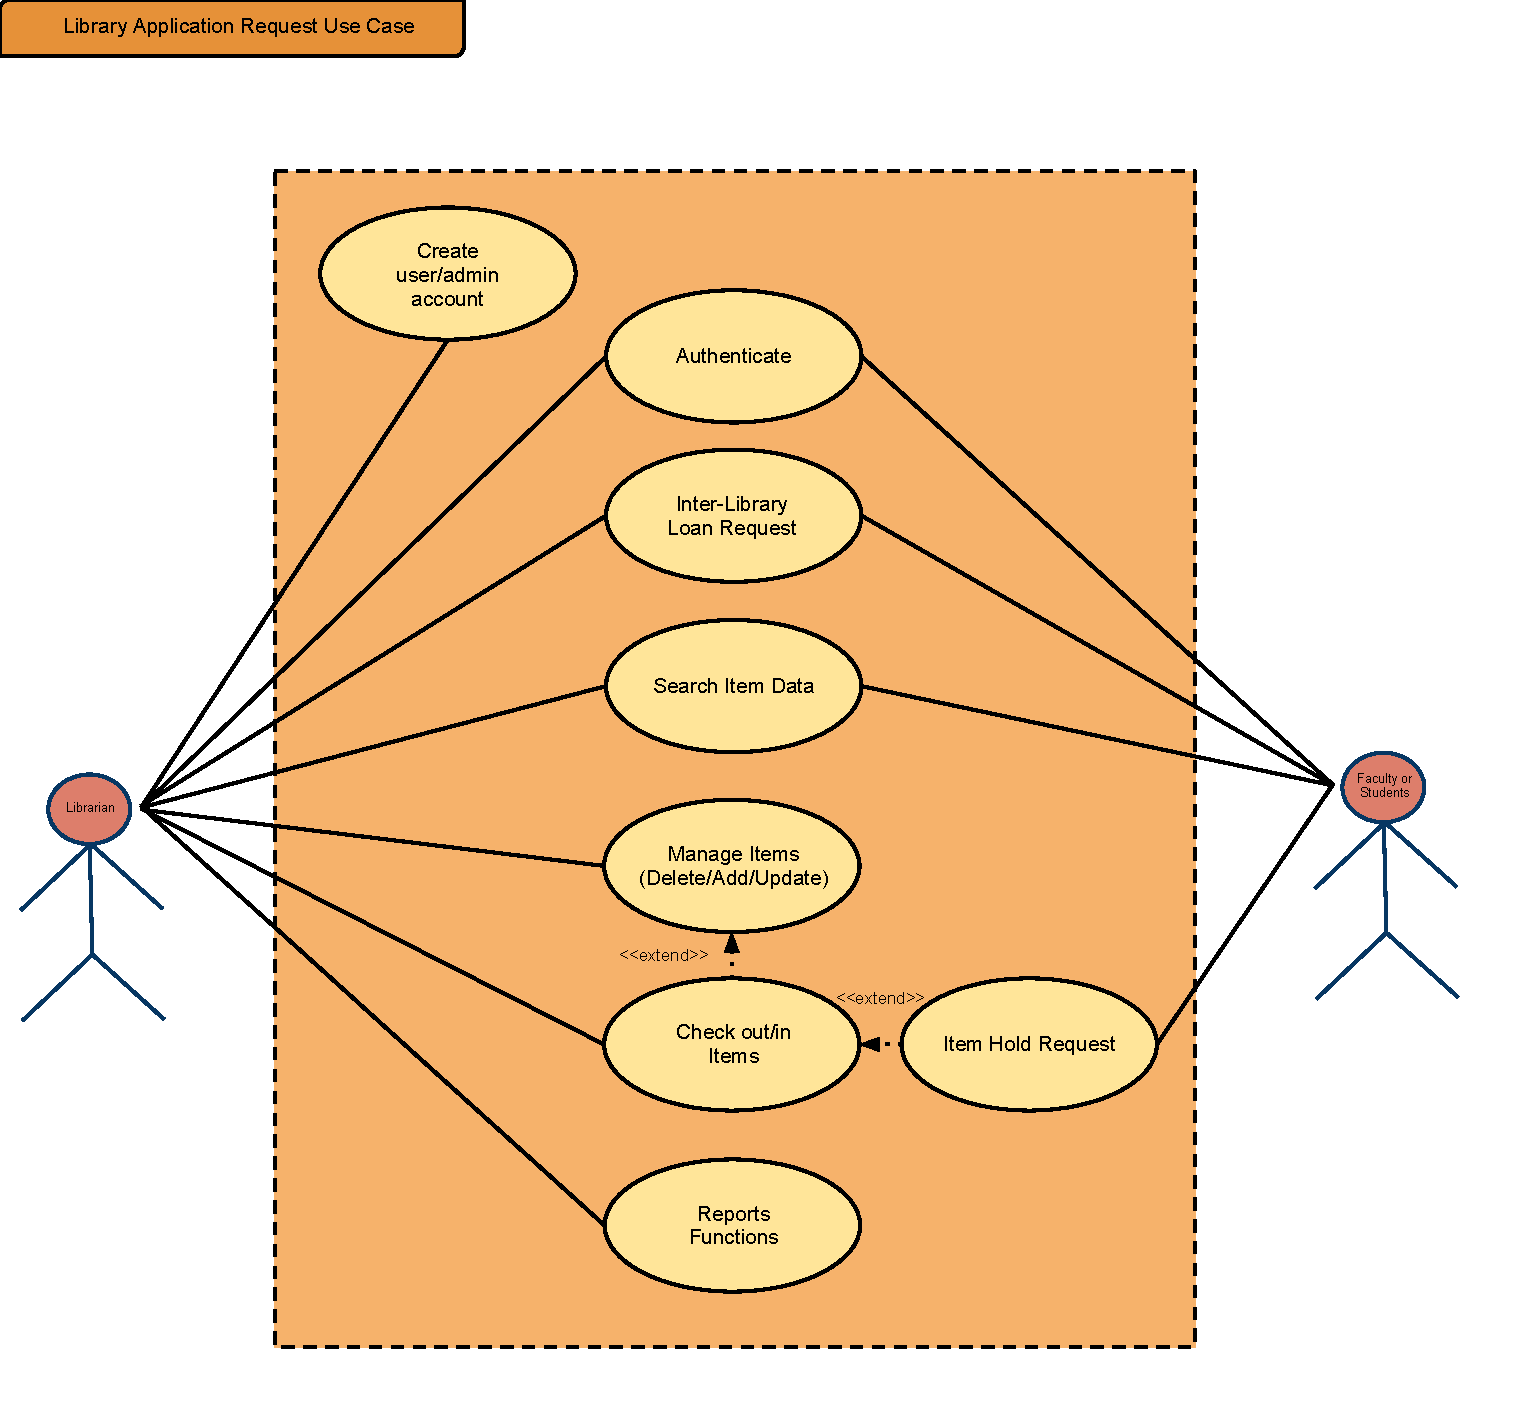
\includegraphics[scale=0.5]{CS434-UML-WK1}
\end{figure}
\clearpage
\section{Stakeholders and Interests}
Various local libraries are depending on this application to work from its inception to improve management of their inventory.
\section{Preconditions}
Librarian must be setup with and administrator account and isbn registered in database with providers.
\section{Success Guaranteed}
(post condition) Books are properly in system. 
\section{Main Success Scenario}
\begin{enumerate}
\item Librarian authenticates.
\item Librarian selects new book data.
\item Librarian enters book title, id and isbn.
\item Book data is recognized and appended to inventory.
\end{enumerate}
\section{Extensions}
\subsection{}
\begin{enumerate}
\item Librarian cannot authenticate.
\item Librarian requests admin account.
\end{enumerate}
\subsection{}
\begin{enumerate}
\item Librarian authenticates.
\item Librarian selects new book data.
\item Librarian enters book title, id and isbn.
\item Book data is not recognized and Librarian notified to contact provider.
\end{enumerate}
\section{Special Requirements}
Library must have a Linux/Unix or OSX based computer.
\section{Technology and Data Variation List}
Providers must keep up with new inventory.
\section{Frequency of Occurrence}
Varies by providers.
\section{Open Issues}
No open issues at this time.
\end{document}